\documentclass{beamer}

\usepackage{beamerthemeSingapore}
\usepackage[brazil]{babel}
\usepackage[T1]{fontenc}
\usepackage[utf8]{inputenc}
\usepackage{graphicx}
\usepackage{url}
\usepackage{xcolor}
\usepackage{booktabs}
\usepackage{array}
\usepackage{ragged2e}
\usepackage{etoolbox}
\usepackage{amsmath}
\usepackage{minted}
\usepackage{qrcode}
\usepackage{tikz}
\usetikzlibrary{positioning, arrows.meta, calc}

% Cores do mapa do jogo, as mesmas do enunciado e do visualizador.
\definecolor{comum}{HTML}{C39A1C}
\definecolor{grave}{HTML}{C92F2A}
\definecolor{hospital}{HTML}{1F7A4D}
\definecolor{eq0}{HTML}{2E6FDB}
\definecolor{eq1}{HTML}{E0731F}
\definecolor{rua}{HTML}{ECE9E1}
\definecolor{quarteirao}{HTML}{B9B4A8}

\newcommand{\amostraq}[1]{\tikz[baseline=-0.6ex]\fill[#1] (0,0) rectangle (0.18,0.18);}
\newcommand{\amostrac}[1]{\tikz[baseline=-0.6ex]\fill[#1] (0.09,0.09) circle (0.09);}
\newcommand{\amostraa}[1]{\tikz[baseline=-0.6ex]\draw[#1, line width=0.8pt] (0.09,0.09) circle (0.08);}

\tikzset{
  caixa/.style = {draw=black, rounded corners=2pt, fill=black!5,
    font=\sffamily\scriptsize, align=center, inner sep=4pt,
    minimum height=0.7cm, line width=0.6pt},
  liga/.style = {-{Latex[length=2mm]}, line width=0.8pt},
  % Células do mapa: x cresce para a direita, y para baixo.
  mapa/.style = {x=0.54cm, y=-0.54cm},
  chamado/.style = {inner sep=0pt, minimum size=0.26cm},
  hosp/.style = {text=hospital, font=\bfseries\Large, inner sep=0pt},
  livre/.style = {draw=eq0, line width=1.2pt, circle, inner sep=0pt,
    minimum size=0.26cm},
  passo/.style = {circle, draw=black, fill=white, font=\sffamily\tiny,
    inner sep=1pt},
  cartao/.style = {draw=#1, line width=1.2pt, rounded corners=3pt,
    minimum width=3.6cm, minimum height=2.4cm, align=center,
    font=\sffamily\small},
  lista/.style = {cartao=#1, minimum height=3.2cm, text width=4.2cm,
    align=left, font=\sffamily\footnotesize},
  segmento/.style = {font=\sffamily\tiny, text=white, align=center,
    inner sep=0pt}
}

% Linhas das células do mapa, uma por unidade de coordenada. O grid do TikZ
% usa passo de 1 cm e ignora a escala x e y do estilo mapa.
\newcommand{\grade}{%
  \foreach \x in {0,...,12} \draw[black!15] (\x,0) -- (\x,8);
  \foreach \y in {0,...,8} \draw[black!15] (0,\y) -- (12,\y);}

\setminted{
  fontsize=\footnotesize,
  breaklines=true,
  breakanywhere=true,
  frame=lines,
  framesep=2mm,
  baselinestretch=1.05,
  tabsize=2
}

\apptocmd{\frame}{}{\justifying}{}

\setbeamertemplate{navigation symbols}{}

\title{Trabalho Prático: Central de Despacho}
\author{Prof. Alex Kutzke}
\date{Outubro de 2026}

\begin{document}

% ==========================================
\begin{frame}
	\begin{center}
		\large{Setor de Educação Profissional e Tecnológica}\\
		Tecnologia em Análise e Desenvolvimento de Sistemas\\
		\vspace{1cm}
		\small{DS143 - Estruturas de Dados II}
	\end{center}
	\titlepage
\end{frame}

% ==========================================
\section{O jogo}

\begin{frame}{Central de Despacho}
	\begin{columns}[c]
		\begin{column}{0.6\textwidth}
			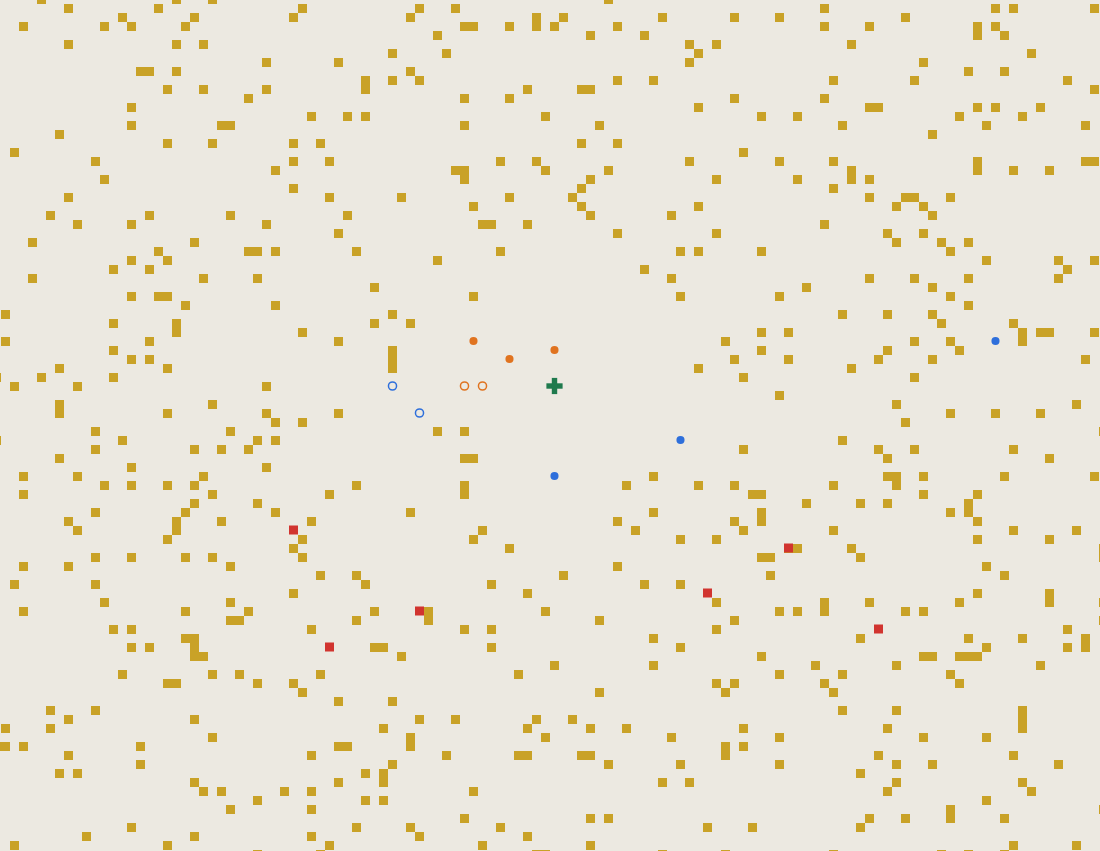
\includegraphics[width=\textwidth]{../img/grade.png}

			\vspace{0.1cm}
			\tiny
			\begin{tabular}{@{}ll@{}}
				\amostraq{comum} chamado comum             & \amostraa{eq0} ambulância livre   \\
				\amostraq{grave} chamado grave             & \amostrac{eq0} ambulância ocupada \\
				\textcolor{hospital}{\textbf{+}} hospital & \amostrac{eq1} outra equipe       \\
			\end{tabular}
		\end{column}
		\begin{column}{0.38\textwidth}
			\small
			Você escreve, em Go, o bot que comanda as ambulâncias.

			\vspace{0.3cm}
			O bot de outra equipe disputa os mesmos pacientes.

			\vspace{0.3cm}
			\textbf{30\% da média}, individual ou em dupla.
		\end{column}
	\end{columns}
\end{frame}

% ==========================================
\begin{frame}{Recolher e entregar}
	\begin{columns}[c]
		\begin{column}{0.6\textwidth}
			\begin{tikzpicture}[mapa]
				\fill[rua] (0,0) rectangle (12,8);
				\grade
				\node[hosp] at (1.5,6.5) {+};
				\node[chamado, fill=comum] at (9.5,3.5) {};
				\node[chamado, fill=grave] at (5.5,3.5) {};
				\node[livre] at (3.5,1.5) {};
				\draw[eq0, dashed, liga] (3.8,1.5) -- (9.5,1.5) -- (9.5,3.2);
				\draw[eq0, liga] (9.5,3.8) -- (9.5,6.5) -- (2.0,6.5);
				\node[passo] at (6.5,1.5) {1};
				\node[passo] at (10.3,3.5) {2};
				\node[passo] at (1.5,7.5) {3};
			\end{tikzpicture}
		\end{column}
		\begin{column}{0.38\textwidth}
			\footnotesize
			\begin{enumerate}
				\itemsep=4pt
				\item A ambulância livre vai ao chamado: $6 + 2 = 8$ turnos, a
				      distância de Manhattan.
				\item Na célula do chamado, recolhe o paciente e fica ocupada.
				\item No hospital, entrega o paciente, e a equipe soma o valor
				      do chamado.
			\end{enumerate}
		\end{column}
	\end{columns}
\end{frame}

% ==========================================
\begin{frame}{Chamados}
	\begin{center}
		\begin{tikzpicture}
			\node[cartao=comum] at (0,0)
			{\textcolor{comum}{\textbf{comum}}\\[4pt]
				95\% dos chamados\\1 a 20 pontos\\prazo longo};
			\node[cartao=grave] at (4.6,0)
			{\textcolor{grave}{\textbf{grave}}\\[4pt]
				5\% dos chamados\\60 a 100 pontos\\prazo curto};
		\end{tikzpicture}
	\end{center}

	\vspace{0.3cm}
	\footnotesize
	\begin{itemize}
		\itemsep=4pt
		\item O servidor avisa quando um chamado é recolhido, por qualquer
		      equipe, e \textbf{não avisa quando ele expira}.
		\item O identificador é sorteado e não serve de índice.
	\end{itemize}
\end{frame}

% ==========================================
\begin{frame}{Um turno}
	\begin{center}
		\begin{tikzpicture}
			\node[caixa, minimum width=2.2cm, minimum height=1.1cm,
				font=\sffamily\small] (s) at (0,0) {servidor};
			\node[caixa, minimum width=2.2cm, minimum height=1.1cm,
				font=\sffamily\small, fill=eq0!15] (b) at (7.4,0) {seu bot};
			\draw[liga] (s.north) to[bend left=25]
			node[above, font=\sffamily\scriptsize, align=center]
				{chamados novos, chamados recolhidos,\\suas ambulâncias, placar}
			(b.north);
			\draw[liga] (b.south) to[bend left=25]
			node[below, font=\sffamily\scriptsize, align=center]
				{um movimento por ambulância:\\
					\texttt{N}, \texttt{S}, \texttt{L}, \texttt{O} ou \texttt{P} (parada)}
			(s.south);
		\end{tikzpicture}
	\end{center}

	\vspace{0.3cm}
	\footnotesize
	O bot tem até 100 ms de processador por turno. O bot ingênuo do kit já
	implementa o protocolo inteiro.
\end{frame}

% ==========================================
\begin{frame}[fragile]{Uma partida}
	\footnotesize
	Na pasta \texttt{ingenuo} do kit:
	\begin{minted}{bash}
go build -o meubot .
../bin/servidor -cenario medio -etapa 1 -semente 7 \
    -replay partida.jsonl ./meubot ../bin/indexado
\end{minted}

	\begin{minted}{text}
Equipe 0 (./meubot): 5615 pontos, 450 recolhidos, ...
Equipe 1 (../bin/indexado): 7415 pontos, 212 recolhidos, ...
\end{minted}

	\vspace{0.1cm}
	O indexado recolheu menos pacientes e fez mais pontos.
\end{frame}

% ==========================================
\begin{frame}{O visualizador}
	\begin{center}
		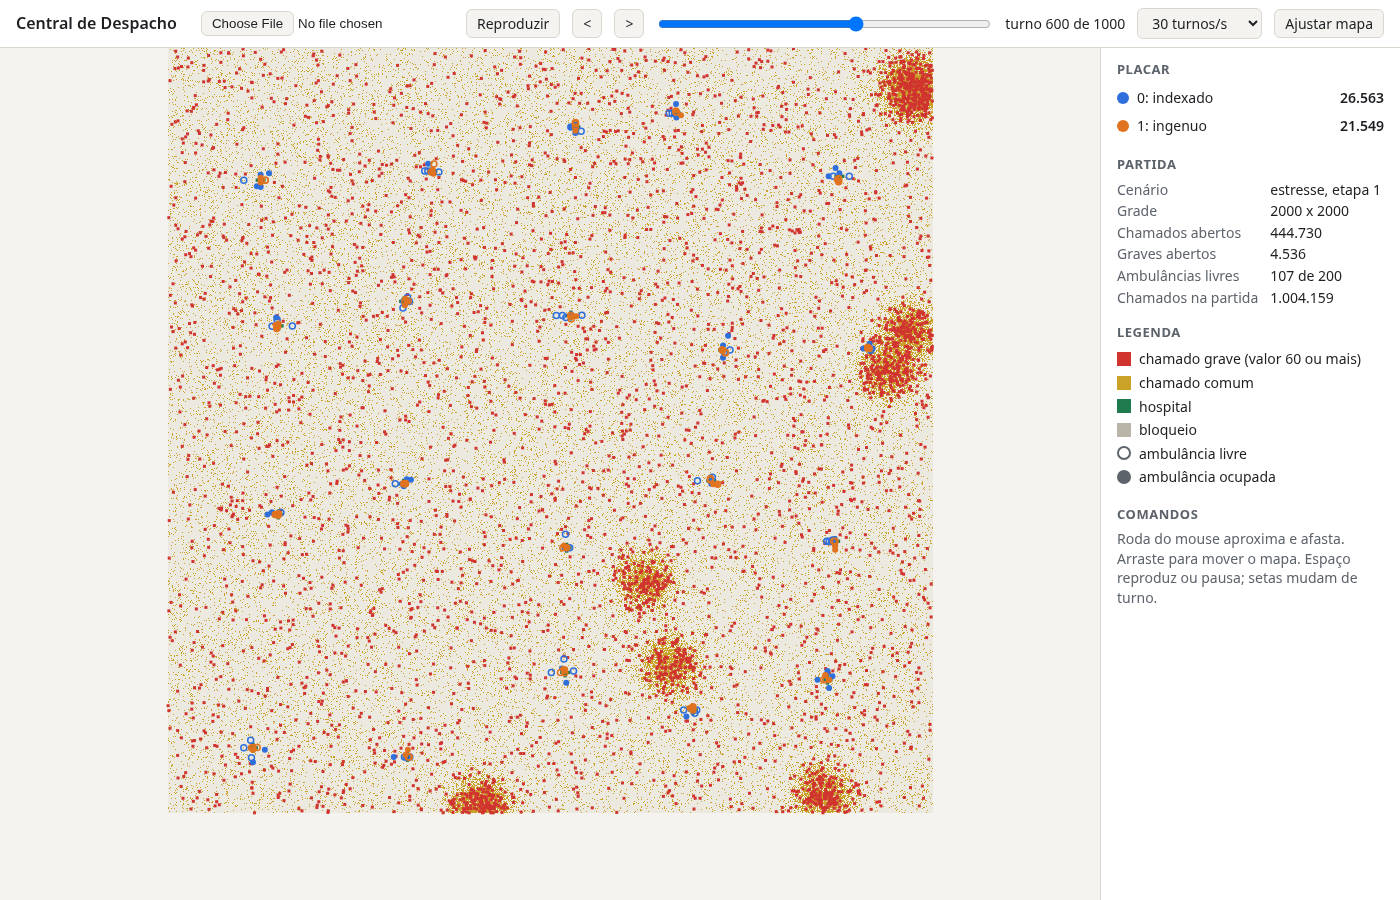
\includegraphics[width=0.92\textwidth]{../img/visualizador.png}
	\end{center}

	\vspace{-0.1cm}
	\footnotesize
	\texttt{visualizador/index.html} no navegador, com o arquivo
	\texttt{partida.jsonl}.
\end{frame}

% ==========================================
\section{Etapas}

\begin{frame}{Etapa 1: o que o seu projeto decide}
	\begin{center}
		\begin{tikzpicture}[op/.style={caixa, text width=2.9cm}]
			\node[draw=comum, fill=comum!20, circle, line width=1pt,
				align=center, font=\sffamily\footnotesize, text width=1.9cm]
			(c) at (0,0) {chamados abertos\\(até 500 mil)};
			\node[op] (o1) at (0,2.4)    {quais estão perto desta ambulância?};
			\node[op] (o2) at (-3.7,0.9) {quais já expiraram?};
			\node[op] (o3) at (-2.7,-1.9) {remover pelo identificador};
			\node[op] (o4) at (2.7,-1.9) {não mandar duas ambulâncias ao mesmo chamado};
			\node[op] (o5) at (3.7,0.9)  {qual o hospital mais próximo?};
			\foreach \o in {o1, o2, o3, o4, o5} \draw[line width=0.6pt] (c) -- (\o);
		\end{tikzpicture}
	\end{center}

	\vspace{0.1cm}
	\footnotesize
	O enunciado não diz quais estruturas usar. Essa escolha é o que o trabalho
	avalia.
\end{frame}

% ==========================================
\begin{frame}{O bot ingênuo no cenário estresse}
	\begin{center}
		\begin{tikzpicture}[x=0.07cm]
			\draw[line width=0.6pt] (0,0) -- (120,0);
			\foreach \v in {0,20,...,120} {
					\draw (\v,0) -- (\v,-0.08);
					\node[below, font=\sffamily\tiny] at (\v,-0.08) {\v};
				}
			\node[below, font=\sffamily\scriptsize] at (60,-0.45)
			{p99 do tempo por turno, em ms};
			\fill[eq1] (0,1.7) rectangle (114.03,2.4);
			\fill[eq0] (0,0.6) rectangle (1.85,1.3);
			\node[left, font=\sffamily\scriptsize] at (0,2.05) {ingênuo};
			\node[left, font=\sffamily\scriptsize] at (0,0.95) {indexado};
			\node[left, font=\sffamily\scriptsize, text=white] at (114.03,2.05) {114,03 ms};
			\node[right, font=\sffamily\scriptsize] at (8.5,0.95) {1,85 ms};
			\draw[grave, dashed, line width=0.8pt] (100,0) -- (100,3.0)
			node[above, font=\sffamily\scriptsize] {teto: 100 ms};
			\draw[hospital, dashed, line width=0.8pt] (7.4,0) -- (7.4,3.0)
			node[above, font=\sffamily\scriptsize, align=center]
				{limite do teste: 4 vezes o indexado};
		\end{tikzpicture}
	\end{center}

	\vspace{0.2cm}
	\footnotesize
	O bot ingênuo guarda os chamados num slice e percorre todos a cada turno.
	Nesta partida, ele passou do teto em 80 turnos.

	\vspace{0.1cm}
	\scriptsize
	p99: tempo abaixo do qual ficam 99\% dos turnos. Semente 3, no computador
	da correção.
\end{frame}

% ==========================================
\begin{frame}{Etapa 2: quarteirões e ruas fechadas}
	\begin{columns}[c]
		\begin{column}{0.6\textwidth}
			\begin{tikzpicture}[mapa]
				\fill[rua] (0,0) rectangle (12,8);
				\fill[quarteirao] (3,2) rectangle (6,8);
				\grade
				\node[livre] (a) at (1.5,4.5) {};
				\node[chamado, fill=comum] at (7.5,4.5) {};
				\draw[grave, dashed, liga] (1.8,4.5) -- (7.2,4.5);
				\draw[eq0, liga] (1.5,4.2) -- (1.5,1.5) -- (7.5,1.5) -- (7.5,4.2);
				\node[font=\sffamily\scriptsize, text=grave, fill=white,
					inner sep=1.5pt, rounded corners=1pt] at (4.5,5.4) {Manhattan: 6};
				\node[font=\sffamily\scriptsize, text=eq0, above] at (4.5,1.5)
				{caminho real: 12};
			\end{tikzpicture}
		\end{column}
		\begin{column}{0.38\textwidth}
			\footnotesize
			O caminho mais curto contorna os bloqueios. Achá-lo é um percurso
			em largura no grafo das células livres.

			\vspace{0.3cm}
			Calcular a cada turno, ou calcular nos 2 s de preparo e guardar,
			com 512 MB de memória?
		\end{column}
	\end{columns}
\end{frame}

% ==========================================
\begin{frame}{Um mapa da etapa 2}
	\begin{center}
		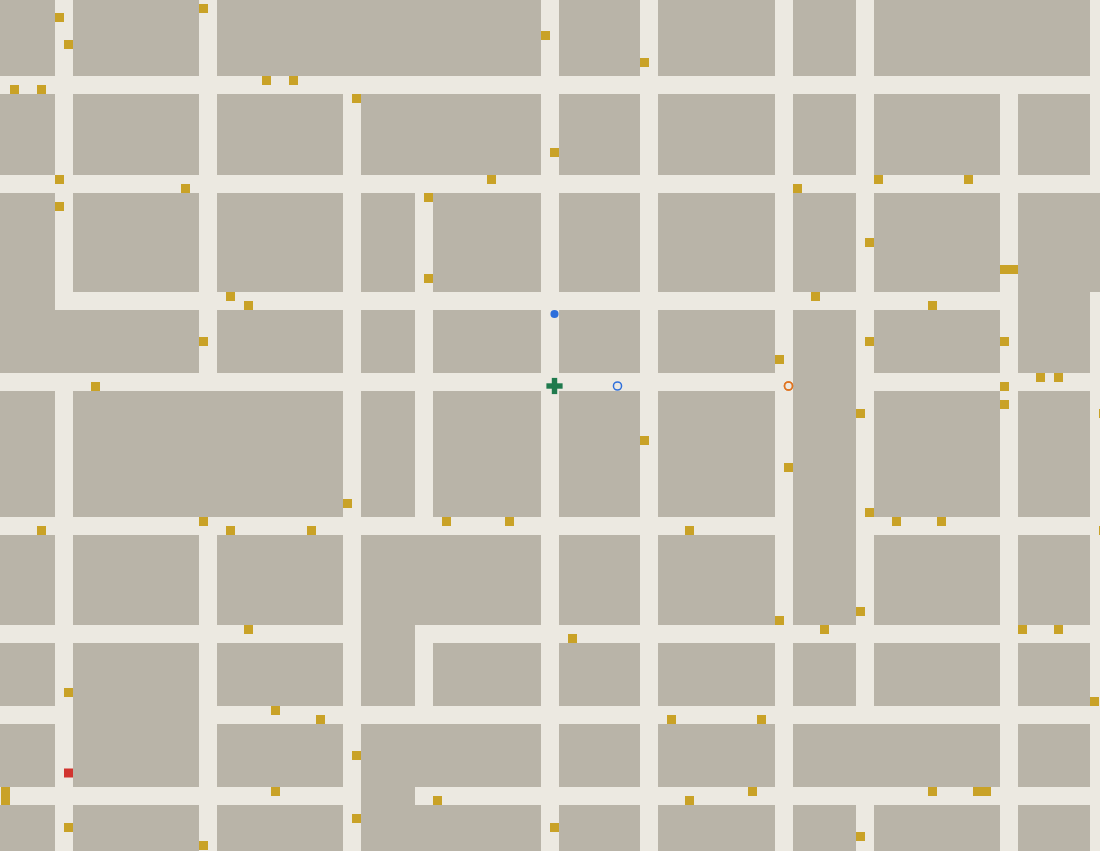
\includegraphics[height=0.68\textheight]{../img/etapa2.png}
	\end{center}

	\footnotesize
	Grafos começam em 04/11. A etapa 1 não depende deles e pode começar já.
\end{frame}

% ==========================================
\section{Kit}

\begin{frame}[fragile]{O kit}
	\begin{center}
		\begin{tikzpicture}
			\node[caixa, fill=eq0!15] (m) at (0,0.5) {seu bot};
			\node[caixa, fill=eq1!15] (i) at (0,-0.5) {bot de referência};
			\node[caixa] (s) at (2.9,0) {servidor};
			\node[caixa] (p) at (5.4,0) {\texttt{partida.jsonl}};
			\node[caixa] (v) at (8.2,0) {visualizador\\(navegador)};
			\draw[liga] (m) -- (s);
			\draw[liga] (i) -- (s);
			\draw[liga] (s) -- (p);
			\draw[liga] (p) -- (v);
			\node[caixa, fill=eq0!15] (e) at (0,-2) {sua entrega};
			\node[caixa] (c) at (2.9,-2) {corretor};
			\node[caixa] (r) at (5.9,-2) {pontos estimados\\(sementes de treino)};
			\draw[liga] (e) -- (c);
			\draw[liga] (c) -- (r);
		\end{tikzpicture}
	\end{center}

	\begin{minted}{bash}
../bin/corretor -etapa 1 -sementes 1-10 -bin ../bin .
\end{minted}

	\footnotesize
	Versões para Linux, Windows, macOS e Docker. As de Windows e macOS, e a de
	Docker fora do Linux, não foram testadas: rode nesta semana e avise o que
	falhar.
\end{frame}

% ==========================================
\begin{frame}{Proibido e permitido}
	\begin{center}
		\begin{tikzpicture}
			\node[lista=grave] at (0,0) {%
				\textcolor{grave}{\textbf{proibido}}\\[4pt]
				o tipo \texttt{map}\\[2pt]
				\texttt{container/heap}\\
				\texttt{container/list}\\
				\texttt{container/ring}\\[2pt]
				bibliotecas de terceiros};
			\node[lista=hospital] at (5.2,0) {%
				\textcolor{hospital}{\textbf{permitido}}\\[4pt]
				o resto da biblioteca padrão\\[2pt]
				o seu código das atividades avaliativas, como a AVL e a tabela
				de hoje};
		\end{tikzpicture}
	\end{center}

	\vspace{0.4cm}
	\footnotesize
	O corretor procura os usos proibidos. Uso encontrado zera os testes de
	pontuação da etapa.
\end{frame}

% ==========================================
\section{Avaliação}

\begin{frame}{Duas modalidades}
	\begin{center}
		\begin{tikzpicture}[x=0.075cm]
			\node[left, font=\sffamily\small] at (0,1.6) {sem IA};
			\fill[eq0] (0,1.25) rectangle (60,1.95);
			\fill[hospital] (60,1.25) rectangle (70,1.95);
			\fill[eq1] (70,1.25) rectangle (100,1.95);
			\node[segmento] at (30,1.6) {suíte 60};
			\node[segmento] at (65,1.6) {10};
			\node[segmento] at (85,1.6) {defesa 30};
			\node[font=\sffamily\tiny, above] at (65,1.95) {relatório};
			\node[right, font=\sffamily\small\bfseries] at (100,1.6) {100};

			\node[left, font=\sffamily\small] at (0,0.35) {com IA};
			\fill[eq0] (0,0) rectangle (60,0.7);
			\node[segmento] at (30,0.35) {suíte 60};
			\node[right, font=\sffamily\small\bfseries] at (60,0.35) {60};
		\end{tikzpicture}
	\end{center}

	\vspace{0.3cm}
	\begin{center}
		\begin{tikzpicture}
			\node[draw=grave, line width=1.2pt, rounded corners=3pt,
				align=center, inner sep=6pt, font=\sffamily\footnotesize]
			{\textcolor{grave}{\Large\textbf{21/10}}\\[3pt]
				declaração de uso de IA, no UFPR Virtual\\
				não pode ser mudada; sem declaração, o trabalho fica com IA};
		\end{tikzpicture}
	\end{center}

	\vspace{0.1cm}
	\scriptsize
	Quem declarar sem IA e não conseguir explicar o próprio código na defesa
	fica com nota máxima 50.
\end{frame}

% ==========================================
\begin{frame}{Suíte de testes}
	\begin{center}
		\begin{tikzpicture}[x=0.16cm]
			\node[left, font=\sffamily\small] at (0,1.9) {etapa 1};
			\fill[eq0!70] (0,1.4) rectangle (10,2.4);
			\fill[eq0] (10,1.4) rectangle (25,2.4);
			\fill[eq0!70] (25,1.4) rectangle (35,2.4);
			\fill[eq0] (35,1.4) rectangle (45,2.4);
			\node[segmento] at (5,1.9) {protocolo\\10};
			\node[segmento] at (17.5,1.9) {tempo\\15};
			\node[segmento] at (30,1.9) {contra o\\ingênuo\\10};
			\node[segmento] at (40,1.9) {contra o\\indexado\\10};
			\node[right, font=\sffamily\small\bfseries] at (45,1.9) {45};

			\node[left, font=\sffamily\small] at (0,0.5) {etapa 2};
			\fill[eq1!80] (0,0) rectangle (7,1);
			\fill[eq1] (7,0) rectangle (15,1);
			\node[segmento] at (3.5,0.5) {protocolo\\e tempo\\7};
			\node[segmento] at (11,0.5) {contra a\\referência\\8};
			\node[right, font=\sffamily\small\bfseries] at (15,0.5) {15};
		\end{tikzpicture}
	\end{center}

	\vspace{0.3cm}
	\footnotesize
	Cada teste joga 10 partidas do seu bot contra um bot de referência.

	\vspace{0.2cm}
	Tempo: o p99 do seu bot até 4 vezes o do bot de referência, na mesma
	partida.

	\vspace{0.2cm}
	Pontuação: a soma de pontos do seu bot acima da do bot de referência, com
	margem de 2\% a 10\%.
\end{frame}

% ==========================================
\begin{frame}{Prazos}
	\begin{center}
		\begin{tikzpicture}[x=1.8cm]
			\draw[line width=1pt, -{Latex[length=2mm]}] (-0.4,0) -- (5.4,0);
			\foreach \i/\data/\texto in {
					0/14\slash10/kit,
					1/21\slash10/declaração\\de IA,
					2/11\slash11/etapa 1 e\\relatório,
					3/25\slash11/Prova 2,
					4/29\slash11/etapa 2,
					5/02\slash12/defesa\\(sem IA)} {
					\fill (\i,0) circle (2.5pt);
					\node[above, font=\sffamily\small\bfseries] at (\i,0.1) {\data};
					\node[below, font=\sffamily\scriptsize, align=center]
					at (\i,-0.1) {\texto};
				}
		\end{tikzpicture}
	\end{center}

	\vspace{0.2cm}
	\footnotesize
	\begin{itemize}
		\itemsep=3pt
		\item Não há entrega com atraso. As tarefas fecham às 23h59.
		\item Em dupla, as duas pessoas enviam a declaração e o arquivo.
		\item Torneio com os bots da etapa 2: os dois primeiros sem IA ganham 5
		      pontos.
	\end{itemize}
\end{frame}

% ==========================================
\begin{frame}{Enunciado completo}
	\begin{center}
		\qrcode[height=4.2cm]{https://tads-ufpr-alexkutzke.github.io/ds143-material/trabalho_2026_02/}

		\vspace{0.4cm}
		\scriptsize
		\url{https://tads-ufpr-alexkutzke.github.io/ds143-material/trabalho_2026_02/}
	\end{center}
\end{frame}

\end{document}
